\chapter{Introduction}\label{introduction}
//TODO Write what is NLP

\chapter{Dialogue systems}\label{dialogue systems}
Dialogue system is a computer system to communicate with a human. Nowadays you meet dialog systems everywhere. A lot of devices have incorporated goal-oriented spoken dialogue systems, such as  Yandex’s Alisa,  Apple’s Siri, Microsoft’s Cortana, Amazon Alexa, and Google Assistant. Dialogue systems are also used in cars (hands-free car-specific functions, Android Auto, Apple CarPlay, vendor-specific solutions), web (search assistants (IKEA), Facebook Messenger and Telegram chatbots), robots, computer games, research systems (skylar.speech.cs.cmu.edu) etc, because a conversation is a natural way for people to get information.

\textbf{Basic Dialogue System Types}:
\begin{itemize}
  \item Task-oriented 
    \begin{itemize}
      \item focused on completing a certain task(s)
    \end{itemize}
  \item Non-task-oriented
    \begin{itemize}
      \item chitchat
      \item gaming the Turing test
    \end{itemize}    
\end{itemize}

\textbf{Communication Domains}:

"\textbf{Domain}" is a conversation topic or an area of interest
\begin{itemize}
  \item Single/Closed-domain is one well-defined area
  \item Multi-domain is joining several single-domain systems
  \item Open-domain “responds to anything”
\end{itemize}


Exists several \textbf{modes of communication}:
\begin{itemize}
  \item Text
  \item Voice
  \item Multimodal
    \begin{itemize}
      \item voice/text + graphics
      \item additional modalities: video - gestures, mimics; touch
    \end{itemize}
\end{itemize}

\textbf{Dialogue initiative}:
\begin{itemize}
  \item system-initiative
    \begin{itemize}
      \item system asks questions, user must reply in oreder to progress
      \item least natural
      \item "form-filling" ("Hello, please enter your e-mail") 
    \end{itemize}
  \item user-initiative
    \begin{itemize}
      \item user asks, machine responds ("Siri, set the timer for 5 minutes")
    \end{itemize}
  \item mixed-initiative
    \begin{itemize}
      \item system and user both can ask and react to queries
      \item most natural
    \end{itemize}
\end{itemize}

\textbf{Dialogue system architecture} is illustrated in Figure \ref{ds architecture}. This architecture consists from Natural Language Understanding (NLU), dialogue management (DM), and Natural Language Generation (NLG).

\textbf{NLU} extracts the meaning from the user utterance and converts into a structured semantic representation. Natural Language Understanding traditionally consists of domain identification and intent prediction, which are framed as utterance classification problems, and slot filling, framed as a sequence tagging task.

\textbf{DM} plays two roles,tracking the dialogue state and performing the dialogue policy (i.e., telling the agent how to act given the dialogue state.)

\textbf{NLG} transforms structured data into natural language.\cite{open_domain_neural_ds}
\begin{figure}[hbt]
  \centering
  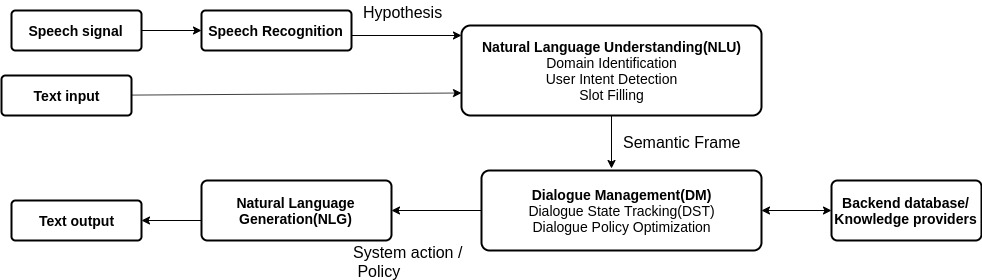
\includegraphics[width=0.8\textwidth]{figures/ds_arcitecture.jpg}
  \caption{Dialogue system architecture.}
  \label{ds architecture}
\end{figure}

\chapter{Natural Language Generation}\label{nlg}
Natural Language Generation is a subsection of Natural Language Processing (NLP). 
NLG approaches can be grouped into two categories, one focuses on generating text using templates or rules (linguistic) methods, the other uses corpus-based statistical methods. 

There is one obvious disadvantage in \textbf{template-based generation}: the quality of the output depends entirely on the set of templates. Even in a relatively  simple domain the number of templates necessary for reasonable quality can become a serious problem.

In \textbf{corpus-based generation} it is possible directly mimicking the language of a real domain expert, rather than attempting to model it by rule, but a good corpus is necessary.
\cite{stochastic_language_generation_ds}

\chapter{Other}
Oh and Rudnicky showed that stochastic generation benefits from two factors: 
\begin{itemize}
  \item it takes advantage of the practical language of a domain expert instead of the developer
  \item it restates the problem in terms of classification and labeling, where expertise is not required for developing a rule-based generation system
\end{itemize}

//TODO: more information in article []
//TODO: Info about datasets
//TODO: NLP vs Computation linguistic

//TODO: In non task oriented dialogue systems it is very difficult to use template-based generation
\cite{stochastic_language_generation_ds}
